\section{Aufbau und Durchführung}

Im ersten Teil des Versuchs wird die Leerlaufspannung $U_\text{0}$ mithilfe eines Voltmeters gemessen.
Danach wird die in Abbildung \ref{fig:A1} gezeigte Schaltung zur Bestimmung des Innenwiderstandes aufgebaut.
\begin{figure}
  \centering
  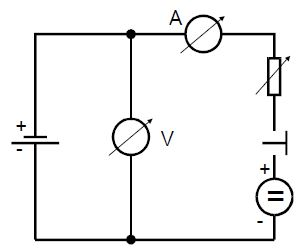
\includegraphics{Text/Bilder/A1.jpg}
  \caption{Messschaltung zur Bestimmung von $U_\text{0}$ u. $R_\text{i}$ \cite[215]{sample}}
  \label{fig:A1}
\end{figure}
Der Belastungswiderstand ist von $\SI{0}{\ohm} - \SI{50}{\ohm}$ regelbar und
wird in regelmäßigen Abständen variiert.
Es werden 10-20 Wertepaare für Stromstärke und Klemmenspannung notiert.
Nach abgeschlossener Messung wird - entsprechend der Abbildung \ref{fig:A2} - zusätzlich eine Gegenspannung
in die Schaltung eingebaut.
\begin{figure}
  \centering
  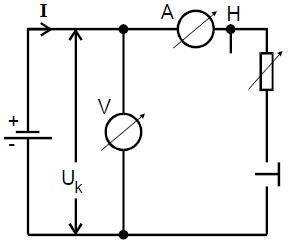
\includegraphics{text/Bilder/A2.jpg}
  \caption{wie Abb.\ref{fig:A1} jedoch mit Verwendung einer Gegenspannung \cite[215]{sample}}
  \label{fig:A2}
\end{figure}
Diese soll \SI{2}{V} größer sein als $U_0$. Der Widerstand wird erneut variiert und 10-20 Messpaare werden notiert.
Der Strom fließt nun in die andere Richtung und es gilt
\begin{equation}
  U_\text{k}=U_\text{0}+I\cdot R_\text{i} .\label{eqn:A2}
\end{equation}
Nun wird die zweite Spannungsquelle wieder ausgebaut, sodass wieder eine Schaltung wie in Abbildung \ref{fig:A1} vorliegt.
Die Monozelle wird nun allerdings gegen einen Sinus- bzw. Rechteckgenerator getauscht.
Ebenso wird hier für die Rechteckspannung ein regelbarer Widerstand von $\SI{20}{\ohm} - \SI{250}{\ohm}$
und für die Sinusspannung ein regelbarer Widerstand von $\SI{0,1}{\kilo \ohm}-\SI{5}{\kilo \ohm}$ verwendet.
Erneut werden pro Spannungsgenerator 10-20 Wertepaare aufgenommen und notiert.
